\section*{Chapter 5}

\subsection*{Exercise 5.1}
Consider the diagrams on the right in Figure 5.1. Why does the estimated
value function jump up for the last two rows in the rear? Why does it drop off for the
whole last row on the left? Why are the frontmost values higher in the upper diagrams
than in the lower?

\subsubsection*{Solution:}

The estimated value function jumps up for the last two rows in the rear because the player has a high probability of winning at 20 and 21, as the dealer is likely to have lower value or go bust.

It drops off for the whole last row on the left because having an ace is a big advantage, thus if the dealer has an ace the probability of the player winning is less.

The frontmost values are higher in the upper diagrams than in the lower because having an usable ace gives an advantage, as the probability of going bust on the next draw is less.

\subsection*{Exercise 5.2}
Suppose every-visit MC was used instead of first-visit MC on the blackjack
task. Would you expect the results to be very different? Why or why not?

\subsubsection*{Solution:}
It would be similar, as in an episode the probability of visiting the same state twice is very low, so the end results would be almost identical. One such rare case is having two aces, then getting a 10.

\subsection*{Exercise 5.3}
What is the backup diagram for Monte Carlo estimation of $q_\pi$? 

\subsubsection*{Solution:}

\begin{figure}[H]
    \centering
    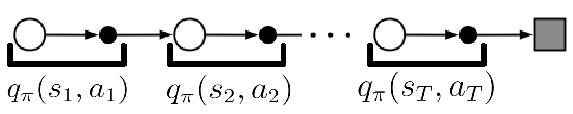
\includegraphics[width=0.8\textwidth]{chapters_latex/figures/ex_05_03.png}
\end{figure}


\subsection*{Exercise 5.4}
The pseudocode for Monte Carlo ES is inefficient because, for each state-
action pair, it maintains a list of all returns and repeatedly calculates their mean. It would
be more efficient to use techniques similar to those explained in Section 2.4 to maintain
just the mean and a count (for each state-action pair) and update them incrementally.
Describe how the pseudocode would be altered to achieve this.

\subsubsection*{Solution:}
We would need to initialize a counter variable $N(s,a) = 0 \quad \forall s \in S, \forall a \in A$, we don't need $\text{Returns}(s,a)$ and $Q(s,a)=0 \quad \forall s \in S, \forall a \in A$. 
In the last step we should have the following:
\begin{itemize}
    \item[] $N(S_t, A_t) \leftarrow N(S_t, A_t) + 1$
    \item[] $Q(S_t, A_t) \leftarrow Q(S_t, A_t) + (G - Q(S_t, A_t))/N(S_t, A_t)$
\end{itemize}

\subsection*{Exercise 5.5}
Consider an MDP with a single nonterminal state and a single action
that transitions back to the nonterminal state with probability $p$ and transitions to the
terminal state with probability $1-p$. Let the reward be $+1$ on all transitions, and let
$\gamma = 1$. Suppose you observe one episode that lasts 10 steps, with a return of 10. What
are the first-visit and every-visit estimators of the value of the nonterminal state?

\subsubsection*{Solution:}
First visit:
\[
    V(S) = 10
\]

Every visit:

\[
    V(S) = \frac{10 + 9 + \dots + 1}{10} = 5.5
\]

\subsection*{Exercise 5.6}
What is the equation analogous to (5.6) for $\textit{action}$ values $Q(s, a)$ instead of
state values $V(s)$, again given returns generated using $b$?

\subsubsection*{Solution:}
\[
    Q(s,a) = \frac{\sum_{t \in \mathcal{T}(s,a)} \rho_{t+1:T(t)-1} G_t}{\sum_{t \in \mathcal{T}(s,a)} \rho_{t+1:T(t)-1}}
\]
 
Where $\mathcal{T}(s,a)$ are the timesteps where action $a$ was takein in state $s$.


\subsection*{Exercise 5.7}
In learning curves such as those shown in Figure 5.3 error generally decreases
with training, as indeed happened for the ordinary importance-sampling method. But for
the weighted importance-sampling method error first increased and then decreased. Why
do you think this happened? 

\subsubsection*{Solution:}

In the beginning there are no good samples, so the estimate is 0. After the first usable sample the estimate might be -1, 0 or 1. This increases the MSE of a single run. In the first 10 episodes more and more runs get their first usable samples, so on average the MSE also increases.

\subsection*{Exercise 5.8}
The results with Example 5.5 and shown in Figure 5.4 used a first-visit MC
method. Suppose that instead an every-visit MC method was used on the same problem.
Would the variance of the estimator still be infinite? Why or why not? 

\subsubsection*{Solution:}

Yes, it would still be infinite. Following the proof in the book, instead of at length $n$ only considering that episode consisting of $n$ timesteps, we should take average of all subsamples in that episode. As the importance of the last timestep is the least, this average is greater than the value in first-visit example.


\subsection*{Exercise 5.9}
Modify the algorithm for first-visit MC policy evaluation (Section 5.1) to
use the incremental implementation for sample averages described in Section 2.4.

\subsubsection*{Solution:}
\fbox{
\begin{minipage}{0.95\textwidth}
\footnotesize
Input: a policy $\pi$ to be evaluated \\
Initialize:
\begin{itemize}
    \item[] $V(s) \leftarrow 0$, for all $s \in S$
    \item[] $N(s) \leftarrow 0$, for all $s \in S$
\end{itemize}

Loop forever (for each episode):
\begin{itemize}
    \item[] Generate an episode following $\pi$: $S_0, A_0, R_1, S_1, A_1, R_2, \ldots, S_{T-1}, A_{T-1}, R_T$
    \item[] $G \leftarrow 0$
    \item[] Loop for each step of episode, $t = T-1, T-2, \ldots, 0$:
    \begin{itemize}
        \item[] $G \leftarrow \gamma G + R_{t+1}$
        \item[] Unless $S_t$ appears in $S_0, S_1, \ldots, S_{t-1}$:
        \begin{itemize}
            \item[] $N(s) \leftarrow N(s) + 1$
            \item[] $V(S_t) \leftarrow V(S_t) + (G - V(S_t))/N(S_t)$
        \end{itemize}
    \end{itemize}
\end{itemize}
\end{minipage}
}


\subsection*{Exercise 5.10}
Derive the weighted-average update rule (5.8) from (5.7). Follow the pattern of the derivation of the unweighted rule (2.3).

\subsubsection*{Solution:}

\begin{align*}
    V_{n+1} &= \frac{\sum_{k=1}^{n}W_k G_k}{\sum_{k=1}^{n}W_k} \\
    &= \frac{W_{n}G_{n} + \sum_{k=1}^{n-1}W_k G_k}{C_n} \\
    &= \frac{W_{n}G_{n} + V_{n}(C_{n}-W_n)}{C_{n}} \\
    &= V_n + \frac{W_n}{C_n}\left[ G_n - V_n\right]
\end{align*}


\subsection*{Exercise 5.11}
In the boxed algorithm for off-policy MC control, you may have been
expecting the W update to have involved the importance-sampling ratio $\frac{\pi(A_t \mid S_t)}{b(A_t \mid S_t)}$, but
instead it involves $\frac{1}{b(A_t \mid S_t)}$. Why is this nevertheless correct?

\subsubsection*{Solution:}

The policy $\pi$ is greedy, it always chooses the action it thinks is best with probability 1, so  $\pi(A_t \mid S_t) = 1$.


\subsection*{Exercise 5.11: Racetrack (programming)}
Consider driving a race car around a turn
like those shown in Figure 5.5. You want to go as fast as possible, but not so fast as
to run off the track. In our simplified racetrack, the car is at one of a discrete set of
grid positions, the cells in the diagram. The velocity is also discrete, a number of grid
cells moved horizontally and vertically per time step. The actions are increments to the
velocity components. Each may be changed by +1, $-1$, or 0 in each step, for a total of
nine $(3 \times 3)$ actions. Both velocity components are restricted to be nonnegative and less
than 5, and they cannot both be zero except at the starting line. Each episode begins
in one of the randomly selected start states with both velocity components zero and
ends when the car crosses the finish line. The rewards are -1 for each step until the car
crosses the finish line. If the car hits the track boundary, it is moved back to a random
position on the starting line, both velocity components are reduced to zero, and the
episode continues. Before updating the car's location at each time step, check to see if
the projected path of the car intersects the track boundary. If it intersects the finish line,
the episode ends; if it intersects anywhere else, the car is considered to have hit the track
boundary and is sent back to the starting line. To make the task more challenging, with
probability 0.1 at each time step the velocity increments are both zero, independently of
the intended increments. Apply a Monte Carlo control method to this task to compute
the optimal policy from each starting state. Exhibit several trajectories following the
optimal policy (but turn the noise off for these trajectories).

\subsubsection*{Solution:}

See the notebooks.

\begin{figure}[H]
    \centering
    \begin{minipage}[b]{0.35\textwidth}
      \centering
      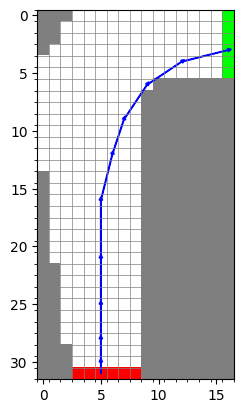
\includegraphics[width=\textwidth]{chapters_latex/figures/ex_05_12_1.png}
      
    \end{minipage}
    \hspace{0.05\textwidth} % Adjusts the horizontal space between images
    \begin{minipage}[b]{0.45\textwidth}
      \centering
      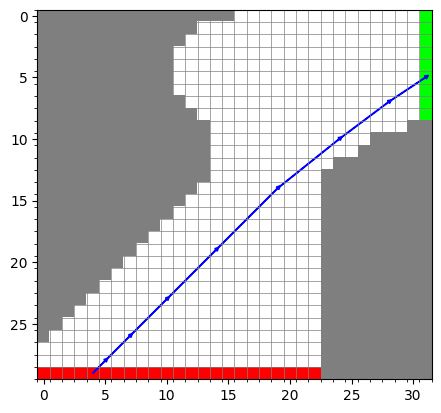
\includegraphics[width=\textwidth]{chapters_latex/figures/ex_05_12_2.png}
    \end{minipage}
  \end{figure}

\subsection*{*Exercise 5.13}
Show the steps to derive (5.14) from (5.12).

\subsubsection*{Solution:}

\begin{multline*}
    \mathbb{E} \left[ \rho_{t:T-1} R_{t+1} \right] = \mathbb{E} \left[ \prod_{k=t}^{T-1} \frac{\pi(A_k \mid S_t)}{b(A_k \mid S_k)} R_{t+1} \right] \\
    = \sum_{A, S, R} \left(\prod_{k=t}^{T-1}\left( p(S_{k+1}, R_{k+1}\mid S_k, A_k) b(A_k \mid S_t) \right) \prod_{k=t}^{T-1} \frac{\pi(A_k \mid S_k)}{b(A_k \mid S_k)} R_{t+1} \right) \\
    = \sum_{A, S, R} \left(\prod_{k=t}^{T-1}\left( p(S_{k+1}, R_{k+1}\mid S_k, A_k) \right) \prod_{k=t}^{T-1} \pi(A_k \mid S_k) R_{t+1} \right) \\
    = \sum_{A, S, R} \left(  R_{t+1} \prod_{k=t}^{T-1}\left( p(S_{k+1}, R_{k+1}\mid S_k, A_k) \right) \prod_{k=t}^{T-1} \pi(A_k \mid S_k) \right) \\
    = \sum_{A_t, S_t, R_{t+1}}   R_{t+1} p(S_{k+1}, R_{t+1}\mid S_t, A_t) \pi(A_t \mid S_t) \\
    = \sum_{A_t, S_t, R_{t+1}}   R_{t+1} p(S_{k+1}, R_{t+1}\mid S_t, A_t) \frac{\pi(A_t \mid S_t)}{b(A_t \mid S_t)} b(A_t \mid S_t)\\
    = \mathbb{E} \left[ \rho_{t:t} R_{t+1} \right] \\
\end{multline*} 


\subsection*{*Exercise 5.14}
Modify the algorithm for off-policy Monte Carlo control (page 111) to use
the idea of the truncated weighted-average estimator (5.10). Note that you will first need
to convert this equation to action values. 

\subsubsection*{Solution:}
We want to achieve this:
\footnotesize
\begin{align*}
Q(s,a) &= \frac{\sum_{t \in \mathcal{T}(s,a)} \left( (1 - \gamma) \textcolor{red}{\sum_{h = t+1}^{T(t) - 1} \gamma^{h - t - 1} \rho_{t:h-1} \bar{G}_{t:h}} + \textcolor{blue}{\gamma^{T(t) - t - 1} \rho_{t:T(t) - 1}} \bar{G}_{t:T(t)} \right)}
{\sum_{t \in \mathcal{T}(s,a)} \left( (1 - \gamma) \textcolor{green}{\sum_{h = t+1}^{T(t) - 1} \gamma^{h - t - 1} \rho_{t:h-1}} + \textcolor{blue}{\gamma^{T(t) - t - 1} \rho_{t:T(t) - 1}} \right)} \\
    &= \frac{\sum_{t \in \mathcal{T}(s,a)} \left( (1 - \gamma) \textcolor{red}{A_t} + \textcolor{blue}{W_t} \bar{G}_{t:T(t)} \right)}
{\sum_{t \in \mathcal{T}(s,a)} \left( (1 - \gamma) \textcolor{green}{B_t} + \textcolor{blue}{W_t} \right)}
\end{align*}

\[
    W_{t-1} = W_t \gamma \frac{1}{b(A_{t-1} \mid S_{t-1})}
\]

\[
    B_{t-1} = (\gamma B_t + 1) \frac{1}{b(A_{t-1} \mid S_{t-1})}
\]

\[
    A_{t-1} = (\gamma A_t + R_{t}) \frac{1}{b(A_{t-1} \mid S_{t-1})} + R_{t-1} B_{t-1}
\]

\fbox{
\begin{minipage}{0.95\textwidth}
\footnotesize
Initialize, for all $s \in S$, $a \in A(s)$:
\begin{itemize}
    \item[] $Q(s, a) \in \mathbb{R}$ (arbitrarily)
    \item[] $C(s, a) \leftarrow 0$
    \item[] $\pi(s) \leftarrow \arg \max_a Q(s, a)$ \hspace{10pt} (with ties broken consistently)
\end{itemize}

Loop forever (for each episode):
\begin{itemize}
    \item[] $b \leftarrow$ any soft policy
    \item[] Generate an episode using $b$: $S_0, A_0, R_1, \ldots, S_{T-1}, A_{T-1}, R_T$
    \item[] $\bar{G} \leftarrow R_T$
    \item[] $W \leftarrow \frac{1}{b(A_{T-1} \mid S_{T-1})}$
    \item[] $A \leftarrow 0$
    \item[] $B \leftarrow 0$
    \item[] Loop for each step of episode, $t = T-1, T-2, \ldots, 0$:
    \begin{itemize}
        \item[] $C(S_t, A_t) \leftarrow C(S_t, A_t) + (1-\gamma)B + W$
        \item[] $Q(S_t, A_t) \leftarrow Q(S_t, A_t) + \frac{(1-\gamma)B + W}{C(S_t, A_t)} [(1-\gamma)A + W \bar{G} - Q(S_t, A_t)]$
        \item[] $\bar{G} \leftarrow \bar{G} + R_{t}$
        \item[] $W \leftarrow W \gamma \frac{1}{b(A_{t-1} \mid S_{t-1})}$
        \item[] $B \leftarrow (\gamma B + 1) \frac{1}{b(A_t \mid S_t)}$
        \item[] $A \leftarrow (\gamma A + R_t)\frac{1}{b(A_t \mid S_t)} + R_{t-1}B $
        \item[] $\pi(S_t) \leftarrow \arg \max_a Q(S_t, a)$ \hspace{10pt} (with ties broken consistently)
        \item[] If $A_t \neq \pi(S_t)$ then exit inner Loop (proceed to next episode)
        
    \end{itemize}
\end{itemize}
\end{minipage}
}


